\section*{\centering Chapter Three}
\section*{\centering Literature Review}
%\addcontentsline{toc}{section}{Chapter Three}
\addcontentsline{toc}{section}{Chapter Three: Literature Review}
The chapter begins with the conceptual framework, showing the causal logic behind the impact of ODA on health outcomes. The causal chain is further contextualised within the existing body of knowledge, , particularly the relations between the variables of interest and this is organized in line with the research questions. The chapter ends with a summary and conclusion of the literature review. 

\subsection*{3.1 Conceptual/Theoretical Framework}
\addcontentsline{toc}{subsection}{3.1 Conceptual/Theoretical Framework}
The major study variables are the ODA (particularly total and social infrastructure ODA), health outcome \footnote{which is proxy by a composite index with indicators from SDG 3 and SDG 2.1 focusing on health and nutrition respectively}, and social protection \footnote{which is proxy by a composite index created from the social protection floor indicators SDG 1.3.1}, as well as a host of other variables perceived to influence the ODA effect on health outcome (see Chapter Four: Methodology, for more details). ODA is the main predictor variable while health outcome is the main dependent variable and social protection is the mechanism through which the effect of ODA partially or completely improves health outcomes. 
The underlying assumption is that a lack of investment, particularly due to insufficient savings in developing countries, hampers their capacity to provide adequate health and social infrastructures for their populations. Consequently, this results in poor health outcomes and a burden of disease \parencite[]{gama_health_2015}, such as a high level of child and maternal mortality, HIV and tuberculosis. Therefore, ODA presents an alternative investment capital to domestic savings and is expected to enhance health capital and overall health outcome in developing countries \parencite{sachs_case_2014, temple_aid_2010}. This assumption is expressed in the causal chain shown in Figure \ref{fig:Causal graph} below:

\begin{figure}[ht]
\captionsetup{justification=justified,singlelinecheck=false}
\caption{\textit{Causal Chain of ODA Impact on Health Outcome}}
    \centering 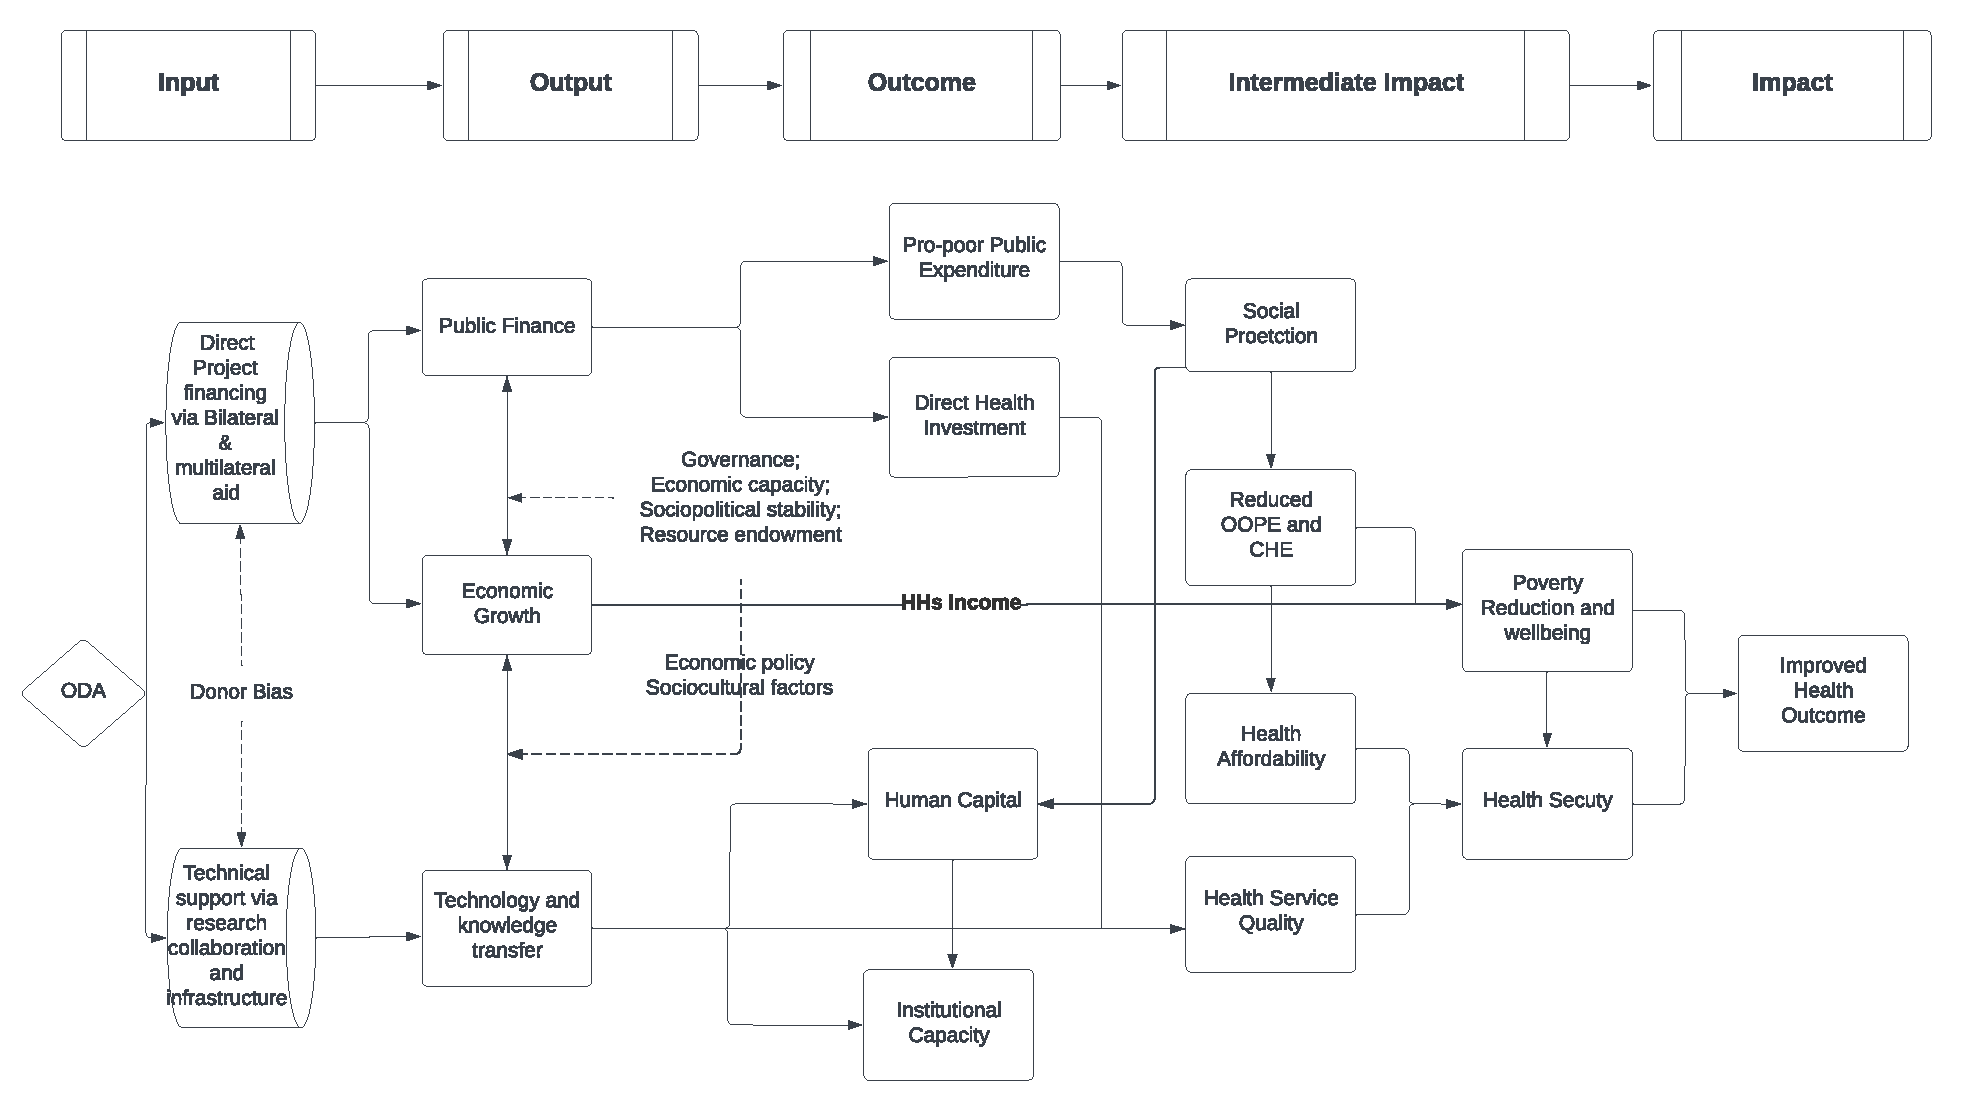
\includegraphics[width = \textwidth]{Figures/Frameworks/Causal Chain Graph for Thesis.pdf}
    \label{fig:Causal graph}
    \caption*{\footnotesize{Note. All variables with dotted lines are assumed to be endogenous factors, capable of moderating the ODA effectiveness on health outcome.\\ Author's illustration.}}
\end{figure}

The conceptual framework draws insights from two economic theories: the Grossman Health Production Theory \parencite{grossman_concept_1972} and the Harrod-Domar Economic Growth Model \parencite{asimakopulos1986harrod}. These theories are synthesized for a comprehensive analysis of the dynamics surrounding health outcomes and ODA.

The Health Demand Theory is a prominent endogenous growth perspective, elucidating the intricate relationship between health outcomes and economic well-being. At its core, the theory posits health as a commodity, produced and consumed by an economic agent \parencite{grossman_concept_1972}. Economic agents produce and consume health, in return for two utilities: (1) freedom from illness and (2) more capacity to work, thus enhancing productivity. Therefore, to maximize optimal health outcomes, economic agents engage in health investments, through various health inputs \parencite{grossman_concept_1972}. While utility from good health remains an agents' motivation for health investment, the capacity for health investment is constrained by the resources available to the agents.

Despite the theory focusing more on micro-level dynamics, it explains the significance of capacity constraints in shaping health outcomes, particularly in developing countries where limited investment capacity in crucial healthcare and social infrastructures contribute to poor health outcomes. Given that health outcomes are intrinsically linked to capability, as equally emphasized by \textcite{sen_health_1998}, pervasive poor health problems in developing countries impede productivity, perpetuating a cycle of poverty \parencite{staicu2017study}.

At a macro level, the Harrod-Domar Growth Model has been influential in understanding the role of investment in economic growth \parencite{asimakopulos1986harrod}. According to the model and its subsequent extension in the two-gap model, insufficient capital accumulation constrains economic growth in developing countries, constituting a development trap  \parencite[see][]{temple_aid_2010}. Therefore, foreign aid is perceived as alternative investment capital to break the countries free from development mysteries \parencite{sachs_case_2014, staicu2017study, temple_aid_2010}.

\subsection*{3.2 Aid Effectiveness Debate: From Economic Growth to Human Development}
\addcontentsline{toc}{subsection}{3.2 Aid Effectiveness Debate: From Economic Growth to Human Development}

The discourse on aid effectiveness in fostering growth and development in developing countries has been a longstanding and debated topic within academia and international development. Originating from an economic perspective in which development deficit in developing countries is attributed to investment gaps, this viewpoint has become the predominant framework for understanding international development for decades \parencite{thuong_impact_2020}. Since then, the debate has continued, leading to a proliferation of perspectives on aid effectiveness. Early scholars assessing aid effectiveness predominantly concentrated on economic growth, viewing it as a tool for poverty reduction \parencite[see][]{yontcheva_macroeconomic_2006}. \textcite{nwude_official_2020} simplifies the divergent views on aid effectiveness into two categories: aid optimists and aid pessimists. 

Aid optimists, grounded in early economic theories, believed that foreign aid could act as an alternative capital to stimulate economic growth and, consequently, eliminate poverty in poor countries \parencite{temple_aid_2010}. In the 2000s, scholars like \textcite{sachs_case_2014, sachs_geography_2001} were vocal advocates of this perspective. Conversely, aid pessimists, citing the widespread poverty in Africa and South Asia despite decades of aid, contend that aid has been ineffective or has even damaged economic growth in the recipient countries \parencite{easterly_aid_2004, easterly_are_2007, easterly_can_2009}.

Beyond these prevailing viewpoints, \textcite{yontcheva_macroeconomic_2006} classified emerging findings into new group defined as aid conditionality and nonlinearity academia. According to these studies, aid effectiveness is contingent on contextual factors in both the receiving and donor countries. Among the relevant factors observed are recipients' governance, initial economic growth, socio-cultural dynamics, and donor conditionality \parencite{yontcheva_macroeconomic_2006, abate_relationship_2022, nwude_impact_2023, temple_aid_2010}. Today, the terrain of academic argument has been replicated beyond aid effectiveness on economic growth \parencite[see][]{yontcheva_macroeconomic_2006, temple_aid_2010}, to other development indicators, including the Human Development Index (HDI), health, inequality and social development \parencite[i.e.][]{aluko_analysis_2021, habtetsion_impact_2017, shafiullah_foreign_2011}. Since the focus of this thesis is on health outcome, the following section discusses the dynamics of aid effectiveness on health outcome in more detail.


\subsection*{3.3 Effectiveness of ODA on Health Outcome}
\addcontentsline{toc}{subsection}{3.3 Health Outcomes as a Focus of Aid Effectiveness}
In the era of Sustainable Development Goals (SDGs), the global focus on addressing public health issues and inequality has increased ODA to social development sectors, particularly the health sector, as depicted in Figure \ref{fig:ODA sectors commitment} (see discussion in Chapter Two). This shift necessitates investigating whether the renewed development interest has indeed realized the intended benefits on health outcomes in recipient countries. Numerous studies have examined the impact of aid on health outcomes using various health indicators, including traditional indicators like incidence of maternal and child mortality, HIV and Tuberculosis, life expectancy, and immunisation coverage \parencite{nwude_official_2020, yan_mortality_2015, doucouliagos_health_2021, kavakli_us_2022, williamson_foreign_2008}. Other general social development indicators from the HDI \footnote{HDI, as a development index, comprises three dimensions, each measured by distinct indicators: Knowledge measured by education, health measured by life expectancy and wellbeing measured by per capita income. Data is computed by UNDP} \parencite{kavanagh_governance_2019, chung_economic_2022, mohamed_foreign_2017} to health promotion research \parencite{cassola_evaluating_2022} have equally been used as measures of health outcome, with inconclusive results. However, it is essential to understand the context of these diverse findings.


\textcite{yan_mortality_2015} assessed the impact of the Global Health Fund, one of the largest multilateral donors in global health, on the rate of change in mortality. The study used all causes of death among adults, under-5 child mortality, and malaria-specific under-five mortality as proxies for mortality. Analyzing data from 1995 to 2010 for all eligible aid countries with fixed effects, the study found a significant positive effect of the Global Health Fund on adult mortality and malaria-specific child mortality. Specifically, an increase of 10 USD in global fund allocation reduced adult mortality and malaria-specific child mortality by 1.4 and 6.9 percent points (p.p) annually \parencite{yan_mortality_2015}. In a similar finding, \textcite{kavanagh_governance_2019} revealed that the global health funding significantly reduces adult mortality, together with the overall HDI, part of which is health. In further macro analysis examining the effect of health aid on infant mortality using fixed effects and two-stage least square with data from 2002 to 2015 for 95 countries, \textcite{doucouliagos_health_2021} revealed that ODA is effective in reducing child mortality.

%%%%%%%%%%% We stopped here with Prof %%%%%%%%%%%%%
In a different study, \textcite{kavakli_us_2022} investigated the impact of the Mexico City Policy (MCP) \footnote{Mexico City Policy (MCP) is a policy in the US, which reduces or removes its ODA for reproductive health promotion, such as access to family planning and abortion \parencite{kavakli_us_2022}}, with data from 1990 to 2015 for 134 countries. Using fixed effects, the authors found that MCP had a significant positive effect on maternal and child mortality as well as HIV incidence, with the impact being more pronounced in countries highly dependent on US aid \parencite{kavakli_us_2022}. These findings are supported by several other studies \parencite{akinola_foreign_2022, mohamed_foreign_2017, muhammad_health_2021, yogo_health_2015}, who have all found the positive impact of ODA on their respective health indicators.

In contrast to the optimistic studies, numerous other investigations have reported the ineffectiveness of aid across various health outcome indicators. One of the earliest pessimistic findings was presented by \textcite{williamson_foreign_2008}. The author assessed the impact of both health and total ODA on health outcomes, utilizing five health indicators: life expectancy, infant mortality, death rate, immunization of measles, and immunization of DPT. The data spanned from 1973 to 2004 and was analyzed using fixed effects. The study concluded that neither total nor health-related ODA significantly influenced health outcomes in developing countries. Instead, only Gross Domestic Product (GDP) was found to significantly reduce infant mortality, with a 1\% increase in GDP leading to a 0.337\% reduction in infant mortality \parencite{williamson_foreign_2008}. More than a decade later, Nwude et al. (2020) supported these findings. Utilizing the Generalized Method of Moments (GMM) to assess the impact of ODA on child mortality and life expectancy, the authors revealed that ODA does not enhance health outcomes. However, control variables such as immunization and the prevalence of HIV were found to influence health outcomes \parencite{nwude_official_2020}. Concentrating on the effect of ODA on Out-of-Pocket Health Expenditure (OOPHE) with data from 1995 to 2015, analyzed with fixed effects and instrumental variables (IV), \textcite{ali_foreign_2020} found no robust effect of ODA on OOPHE. These conclusions are corroborated by various other studies, collectively discrediting the notion of ODA significantly impacting health outcomes \parencite{bavinger_relationship_2017, chung_economic_2022, rosala-hallas_global_2018, toseef_how_2019}.

In the pursuit of understanding aid effectiveness on health outcomes, several studies have ventured into exploring various health-related indicators. In a qualitative study focused on assessing the ODA research grant mechanisms on global health, \textcite{cassola_evaluating_2022} revealed that ODA research grants positively influence the research landscape by elevating research institutions, promoting interdisciplinarity, and increasing the volume of research. However, this effectiveness was observed primarily for donor countries, with no significant evidence of direct welfare development in recipient countries \parencite{cassola_evaluating_2022}. In a different study, \textcite{bavinger_relationship_2017} examined the relationship between child health ODA allocation and the global burden of disease \footnote{The global burden of disease was proxied by vaccine-preventable diseases such as newborn diseases \parencite{bavinger_relationship_2017}}. The authors concluded that there is no significant relationship between child health ODA allocation and the global burden of disease \parencite{bavinger_relationship_2017}.

Amidst the ongoing macro-analysis debate, a parallel exploration of the micro-level impact of ODA has yielded a mix of findings. \textcite{akinola_foreign_2022} directed their analysis towards evaluating the effect of ODA on health outcomes, proxied by life expectancy, in Nigeria, using Auto Regressive Distributive Lag (ARDL). The authors concluded that ODA had no significant effect on life expectancy in Nigeria, with government expenditure emerging as the influential factor. In Uganda, \textcite{odokonyero_impact_2018} investigated how health ODA impacted the prevalence and burden of diseases, utilizing household survey data spanning from 2005 to 2014 through the Difference-in-Difference (DID) approach. Despite the observation that health ODA may not always be allocated to where it is needed the most, the author found that health ODA not only significantly affected the productivity burden of disease but also hastened recovery times rather than preventing diseases. Moreover, aid was found to be more effective for those living close to the project areas \parencite{odokonyero_impact_2018}. 

Conversely, despite using a similar DID method, \textcite{marty_taking_2017} reported 
different findings in Malawi, focusing on the effect of infrastructure and parasitic ODA on the incidence of malaria and perceived adequacy of healthcare with a two-wave household survey in 2010/2011 and 2004/2005. Regardless of foreign aid being less allocated to the least developed areas, infrastructure and parasitic aid were associated with a reduction in malaria prevalence by 1.20 to 12.1 percentage points (Marty et al., 2017). This finding gains additional support from the work of \textcite{muhammad_health_2021}, who, in a study conducted in Nigeria, observed a significant influence of health-related ODA on health outcomes in both the short and long term.

%%%%%%%%%%%%%%%%%%%%%% Conditions moderating ODA %%%%
\subsubsection*{- Conditionality and Nonlinearity of ODA Effectiveness}
\addcontentsline{toc}{subsubsection}{Conditionality and Nonlinearity of ODA Effectiveness}

To address the controversies surrounding the ODA's effectiveness on health outcomes, several studies have delved into explaining the conditions that moderate this impact. \textcite{doucouliagos_health_2021} attributed the mixed or ineffective findings in previous studies to the absence of governance in their models, making governance a crucial moderating variable in the effect of ODA on health. Utilizing fixed effects and two-stage least squares (2SLS) with data spanning from 2002 to 2015 for 95 countries, the authors revealed that the impact of health ODA on infant mortality is contingent on governance, particularly government effectiveness and corruption levels \parencite{doucouliagos_health_2021}.

In a dynamic panel model, \textcite{abate_relationship_2022} demonstrated that the effect of ODA on enhancing economic growth becomes negative only when governance and economic freedom indicators fall below a certain threshold. The author concluded that government effectiveness is essential to observe aid effectiveness. Similarly, to consider the role of government effectiveness and capacity in the effect of ODA on the Human Development Index (HDI), \textcite{chung_economic_2022} interacted their main predictors, ODA and Gross Domestic Product (GDP) per capita. In both models, the study revealed that government effectiveness and capacity magnified the effect of ODA on HDI \parencite{chung_economic_2022}. This finding is supported by \textcite{muhammad_health_2021}, where governance indicators such as government effectiveness, corruption, accountability and voice, rule of law, and regulation quality competitively reduced under-5 child mortality. In their study, \textcite{kavanagh_governance_2019} even asserted that the global health fund reduced child mortality while simultaneously improving government effectiveness, corruption control, and the rule of law. Furthermore, in a systematic study on ODA effectiveness in poverty reduction, \textcite{mahembe_foreign_2019} emphasized the role of democracy in enhancing aid effectiveness.

In contrast, this perspective was debunked over a decade ago by \textcite{williamson_foreign_2008}, who combined five health indicators as outcomes and found that governance indicators, such as the Fraser freedom index and political freedom, did not influence health outcomes \parencite{williamson_foreign_2008}, subsequent studies have reiterated this finding. For instance, in a similar study, \textcite{david_contribution_2017} found governance to be insignificant in moderating ODA effectiveness. This observation was also supported by \textcite{ali_foreign_2020}, where institutional quality was deemed insignificant in influencing health outcomes or the effectiveness of foreign aid on health.

Another dimension to consider is highlighted by \textcite{yogo_health_2015}, who compared the effects of ODA on health outcomes, using HIV incidence, child mortality, and life expectancy as proxies, between post-conflict and stable states. Using a Generalized Method of Moments (GMM) combining both system and first differencing methods, the authors found that ODA significantly improved health indicators in post-conflict states. Similarly, \textcite{bavinger_relationship_2017} suggested that Child Health ODA could have the intended effect if allocated to the burden of diseases. Using quartile regression, \textcite{mohamed_foreign_2017} revealed that the effectiveness of foreign aid was observable in the 25th, 50th, and 75th quantiles, while the effect declined along the ranking, confirming the nonlinearity of aid effectiveness.



\subsection*{3.4 Social Protection's Mediating Role in ODA's Impact on Health Outcomes}
\addcontentsline{toc}{subsection}{3.4 Social Protection's Mediating Role in ODA's Impact on Health Outcomes}
In recent times, the convergence of health economics/public health and social protection has become increasingly prominent, breaking down the silos that traditionally separated these fields. This integration is partly championed by endogenous growth economists such as Grossman (1972), Östlin et al. (2004), A. Sen (1996), K. Sen, and Koivusalo (1998), and Wagstaff (2002), through contributions on poverty, economic conditions and health outcome. Development organizations and scholars have advocated for social protection as a crucial instrument, particularly in advancing Universal Health Coverage (UHC). The rationale is that social protection plays a pivotal role in poverty eradication and reduction, thereby promoting UHC by eliminating financial barriers to healthcare services, ensuring access, affordability, and health equity \parencite{fox_clinical_2015, ilo_towards_2020, lonnroth_beyond_2014, siroka_association_2016, world_bank_high-performance_2019, who_world_2010}.

\subsubsection*{\quad 3.4.1 Social Protection and Health Outcome}
\addcontentsline{toc}{subsubsection}{3.4.1 Social Protection and Health Outcome}

The interconnection between social protection and health has gained momentum, especially in the aftermath of the Covid-19 pandemic \parencite[see][]{mccord_official_2021, yokobori_roles_2023}. One significant consensus from the literature is that social protection contributes to the discourse on public health in two main ways. Firstly, the evolution of social protection has reinforced the realization of a rights-based approach to health, particularly with the integration of health into various social protection frameworks \footnote{A significant example is the ILO Social Protection Floor (SPF recommendation 202), which is now integrated in SDG 1.3} \parencite[discussion in][]{hagemejer_role_2013, ilo_social_2012, macnaughton_decent_2010, ilo_towards_2020, yokobori_roles_2023}. Secondly, and particularly relevant to this thesis, social protection contributes to the development of health financing models, notably social security and social assistance—both integral components of Social Protection \parencite{scheil-adlung_focusing_2020, scheil-adlung_response_2014, world_bank_high-performance_2019, who_world_2010}. Consequently, studies examining the impact of social protection on healthcare outcomes can be categorized into two main groups: those focusing on social insurance and those examining social assistance. While each stream of research offers valuable insights, the evidence remains inconclusive.

\paragraph{\quad \quad \textit{3.4.1.1	Social Insurance and health outcome}} 
\subparagraph{}
Although the impact of social insurance on health outcomes is mixed, with significant controversy around its efficacy in safeguarding vulnerable and impoverished populations from Catastrophic Health Spending (CHS) \parencite{korachais_impact_2019, sarkodie_effect_2021}. The controversy is not surprising, given that the subsidization or elimination of medical user fees might be perceived as a windfall gain, leading to increased utilization of healthcare services in terms of both quantity and quality by households. A systematic review by Azzani and colleagues identified health shocks as a major cause of high health consumption among poor households, thereby inducing CHS \parencite{azzani_determinants_2019}. In a similar study conducted in China, \textcite{xu_equity_2021} reported that poor households disproportionately consumed health services compared to other income groups. This observation may explain the findings of \textcite{helmsmuller_does_2022} in the evaluation of the Social Protection Health Initiative (SPHI) in Pakistan, where despite the provision of free inpatient insurance, the quantity of care remained relatively constant, with most households shifting from public to private healthcare. If social insurance indeed protects freedom of choice and enhances care quality, as reported by \textcite{helmsmuller_does_2022} and others \parencite{gajate2015effect, korachais_impact_2019}, then its impact is noteworthy.

Conversely, other studies have reported the positive impact of social insurance on health outcomes extending beyond freedom of choice. In a study conducted in Vietnam, analyzing survey data from 46,000 households with multivariate regression, \textcite{sepehri_how_2014} concluded that the use of social insurance cards reduced Out-of-Pocket (OOP) health expenditure by 50 to 56\% compared to a counterfactual group. Similarly, in the seventh round assessment of the National Health Insurance Scheme (NHIS) in Ghana, \textcite{sarkodie_effect_2021} reported that NHIS increased health demand by 26\% while reducing OOP spending by 4\%. These findings are complemented by many others \parencite{dror_impact_2016, frolich_effects_2018, habib_role_2016, levine_insuring_2016}, indicating that the provision of health insurance offers financial protection from CHS, improves service access, and leads to various positive social outcomes. In fact, \textcite{dror_impact_2016} conclude that health insurance has the potential to generate welfare gains that could elevate poor households up the income ladder.

 
\paragraph{\quad \quad \textit{3.4.1.2	Social Assistance and Health outcome}}
\subparagraph{}
Social assistance is widely recognized as a set of programs or policies that offer non-contributory transfers, in the form of either or both in-kind and cash assistance, to improve the livelihoods of individuals considered vulnerable or living in chronic poverty \parencite{heggebo_disentangling_2020, shahidi_impact_2019, world_bank_state_2015} \footnote{Social assistance provision serves as protective measure, thus, it means-targetted and could be short term}. Health shocks affect poor individuals in two ways: first, through the financial burden of direct healthcare service costs, and second, through indirect costs resulting from the loss of income due to low productivity or an inability to work \parencite{helmsmuller_does_2022}. Therefore, social assistance provides a safety net, as described by the \textcite{world_bank_state_2015}, protecting the poor and vulnerable during challenging times. Assessing the impact of social assistance on health outcomes is particularly novel.

\textcite{adato_social_2009} summarized the health impact of cash transfers as protecting against the direct costs associated with accessing health services and enhancing self-health management behaviours among the poor through health education and conditional assistance. Similarly, in the review of \textcite{shahidi_impact_2019}, four experimental and quasi-experimental studies found that a reduction in the adequacy of social assistance benefits had adverse health effects, emphasizing the importance of ensuring adequate benefits for optimal outcomes. In Sub-Saharan Africa (SSA), \textcite{owusu-addo_impact_2018} revealed that the provision of cash transfers improved healthcare consumption and financial protection. 
Therefore, social protection, through the combination of different instruments, offers a comprehensive approach to enhancing health outcomes and addressing inequities in health systems \parencite{hagemejer_role_2013, world_bank_high-performance_2019, yokobori_roles_2023, ilo_towards_2020, who_world_2010}. 

\subsubsection*{\quad 3.4.2 ODA Effectiveness on Social Protection:}
\addcontentsline{toc}{subsubsection}{3.4.2 ODA Effectiveness on Social Protection}
Despite its crucial role, establishing a sustainable and stable social protection system requires substantial capital investment, a resource often lacking in developing countries (McCord et al., 2021). As of 2020, the International Labour Organization (ILO) estimated a financing gap of USD 1,191.6 billion or 3.8\% of GDP in low and middle-income countries for social protection floors, including Universal Health Coverage \parencite{duran-valverde_financing_2020}. The demand for ODA is crucial, especially in the COVID-19 pandemic, where an increase in ODA flow has enabled many low-income countries to enhance their social protection systems \parencite{mccord_official_2021}. Despite the growing demand for ODA for social protection, few studies have explored its impact, and existing ones often use general poverty or human development indicators as proxies for social protection \parencite{forte_impact_2023, lonnroth_beyond_2014, mahembe_foreign_2019, shafiullah_foreign_2011}.

Niño-Zarazúa and colleagues conducted a study assessing the effect of ODA on social protection, proxy by coverage of non-contributory programmes, in low and middle-income countries, using an instrumental variable with a Tobit regression model. The findings revealed that ODA has contributed to the expansion of social protection systems in developing countries. Specifically, a 1\% increase in ODA allocated to social protection increased coverage by 0.25\% points, with the highest impact observed in Sub-Saharan Africa (0.26\%) \parencite{nino-zarazua_aids_2023} \footnote{One significant limitation in the study and others aiming to study social protection is the lack of panel data on various social protection performance indicators. Both ILO and World Aspire data are only suitable for cross-sectional analysis \parencite{nino-zarazua_aids_2023}}. A systematic literature review on aid effectiveness in poverty reduction by \textcite{mahembe_foreign_2019} classified studies based on monetary and non-monetary poverty indicators, showing that ODA has contributed to poverty reduction in most studies, regardless of the poverty indicator used. 

\textcite{david_contribution_2017} investigated the effect of ODA on poverty reduction in ECOWAS countries in SSA region, covering data from 1980 to 2014. The study revealed that ODA reduced poverty through the channel of infant mortality. Additionally, both ODA and Foreign Direct Investment (FDI) increased domestic investment in the studied region \parencite{david_contribution_2017}. In a similar study, \textcite{mohamed_foreign_2017} explored the impact of ODA per capita on human welfare, particularly in poverty reduction, using quartile regression. The study found that ODA has a significant impact on human welfare across all quartiles, although the impact is nonlinear. Focusing on the role of ODA in reducing GINI inequality, \textcite{shafiullah_foreign_2011} employed a combination of fixed and random effects. The study found a negative relationship between ODA and inequality, with the conclusion that inequality is inevitable at the initial stages of a country's growth, aligning with the Environmental Kuznets Curve (EKC) hypothesis.

In contrast to the findings above, \textcite{forte_impact_2023} examining the impact of Foreign Direct Investment (FDI) on social welfare, proxied by HDI \footnote{Virtually all studies on Social welfare used HDI, encompassing income, health, and education} data from 2002 to 2019 for 146 countries, found that FDI harmed social welfare and human development. This negative impact was only reversed in countries with already high human capital. The authors concluded that as FDI increases wage inequality, it fails to improve the situation of poor people due to their lack of the required absorptive human capital \parencite{forte_impact_2023}. Similarly, in the work of \textcite{alves_impact_2023}, focusing on the impact of foreign aid on aggregate welfare, proxy by HDI, the authors found no evidence that ODA enhances human development. This finding is consistent with \textcite{gama_health_2015}, who did not identify any significant effect of ODA on African household income, measured by Gross National Income (GNI), or education.

In a quest to assess the competing effect of both FDI and ODA on poverty reduction with data spanning 1990 to 2017 for 29 countries in SSA, \textcite{anetor_impact_2020} found no significant effect of either ODA or FDI on poverty reduction in Africa. The authors concluded that the required amount of FDI for poverty alleviation in Africa has not been reached, and the flow of ODA has not been channelled effectively. Taking a more comprehensive approach, \textcite{iwegbu_effectiveness_2022} reported that foreign aid, when combined with effective fiscal policies on education and health, significantly enhanced household income in all African regions. This underscores the necessity of combining policies for optimal social outcomes. This perspective aligns with the findings of the systematic review by \textcite{mahembe_foreign_2019}, where the authors concluded that ODA allocated to pro-poor sectors, such as education, health, and other social services, proves to be more effective for poverty reduction.



\subsection*{3.5 Regional Heterogeneity of ODA Impact}
\addcontentsline{toc}{subsection}{3.5 Regional Heterogeneity of ODA Impact}
\paragraph{} An entrenched belief in academia that aid ineffectiveness may be specific to certain regions, is repeatedly expressed by \textcite{easterly_can_2009, easterly_aid_2004}, who justified aid ineffectiveness by citing perpetual poverty and state development challenges, particularly in Africa, despite foreign aid. This viewpoint has spurred renewed academic interest in studies controlling for regions when assessing aid effectiveness, yet the pattern of findings remains inconclusive.

In a study by \textcite{yan_mortality_2015} on the impact of the Global Health Fund on adult and child mortality as well as HIV incidence, two models were employed—one comprising all countries and the second restricted to the SSA region. The general model revealed a significant effect of the global health fund on the measured indicators. Specifically, a 10 USD per capita increase in the global health fund is attributed to a 6.9 percentage points reduction in malaria-specific child mortality. However, in the SSA-specific model, the effect was reduced to 3.6 percentage points \parencite{yan_mortality_2015}. Analyzing social protection coverage and ODA with an Instrumental Variable (IV)-Tobit model, \textcite{nino-zarazua_aids_2023} found that the effect of ODA on social protection coverage was the highest in SSA compared to the Pacific, Latin America and the Caribbean (LAC). Specifically, a 1\% increase in ODA allocation increased social protection coverage by 0.26\% in SSA, 0.24\% in the Pacific, and 0.12\% in LAC.

More broadly, \textcite{doucouliagos_health_2021} controlled for dummy variables capturing regional variations across SSA, Middle East and North Africa (MENA), LAC, Europe and Central Asia, South Asia, North America, East Asia and Pacific. Their data, covering 2002 to 2015 for 95 countries, revealed that the effectiveness of foreign aid was observable across regions when conditioned on governance and was not significantly different across regions. Similarly, \textcite{mohamed_foreign_2017}, employing a similar procedure, revealed that aid effectively improved people's income and had the potential for poverty reduction across regions.


In a more comprehensive study focusing on SSA, \textcite{nwude_impact_2023} examined the impact of aid channels, specifically bilateral and multilateral while considering regional differences between Francophone and Anglophone SSA. Using a Pooled Mean Group (PMG) approach, the study revealed that bilateral aid had a positive and significant effect in Francophone SSA, whereas it exhibited a weak negative effect in Anglophone SSA. The negative effect of multilateral aid was stronger in Anglophone SSA compared to Francophone SSA \parencite{nwude_impact_2023}. These findings align with \textcite{yogo_health_2015}, where health ODA significantly reduced child mortality, albeit the impact is more visible in post-conflict states than in stable states. In another study, \textcite{chung_economic_2022} investigated the socioeconomic impact of ODA in Africa using a spatial autocorrelation panel model. They found that ODA had a significant and positive effect on the Human Development Index (HDI), although no effect on GDP per capita.

Contrastingly, \textcite{nwude_official_2020} compared SSA and non-SSA regions in the effect of ODA and income per capita on health outcomes. While health ODA did not improve life expectancy, income per capita did, and this finding was consistent across regions. However, the effect of ODA was reported to be higher in SSA than in non-SSA regions \parencite{nwude_official_2020}. This aligns with \textcite{staicu2017study, gama_health_2015}, who posited that foreign aid does not improve education or household income in Africa. More intricately, \textcite{shafiullah_foreign_2011} evaluated the effect of ODA on inequality reduction, considering regional variation in results. The findings indicated that while the first lag of ODA significantly reduced inequality in the general model, the second lag order of ODA increased inequality in South Asia, with similar findings for GDP. 

\subsection*{3.6 Summary and Conclusions from the Literature Review}
\addcontentsline{toc}{subsection}{3.6 Summary and Conclusions from the Literature Review}
\paragraph{} In summary, the literature review extensively explores the intricate relationship between Official Development Assistance (ODA) and health outcomes, highlighting the potential mediating role of social protection. The debate on aid effectiveness is thoroughly examined, encompassing macro and micro-level analyses with divergent perspectives from optimists and pessimists. The review delves into conditions moderating aid effectiveness, emphasizing the nuanced assessments required, especially in the context of regional variations. Amidst these debates, social protection emerges as a crucial mediator, bridging health and economic well-being. The intersection of poverty and health conditions underscores the role of social protection in promoting health equity. Despite the mixed impact of social insurance in protecting the vulnerable against CHS, both social insurance and social assistance provides the opportunity to enhance health outcome and address health inequity.

As the literature remains inconclusive, the thesis adopts a unique perspective by navigating the complexity of health outcome definitions, considering regional dynamics of health problems, and recognizing the mediating role of social protection. This approach is crucial for understanding aid effectiveness and informing policymaking in the realm of international development. The synthesis of evidence provides a foundation for the empirical investigation within the thesis, aiming to contribute meaningfully to the ongoing discourse on aid impact and health outcomes.